\documentclass{article}
\usepackage[utf8]{inputenc}

\title{623 Project 2: Finite Volume Solver}
\author{Josh Anibal}
\date{February 22nd 2019}

\usepackage{natbib}
\usepackage{graphicx}
\usepackage{pdflscape}
\usepackage{afterpage}
\usepackage{lscape}
\usepackage{amsmath, esint}
\usepackage{geometry}
\geometry{ margin=0.75in}
\usepackage[utf8]{inputenc}
\usepackage[english]{babel}

\usepackage{floatrow}
% Table float box with bottom caption, box width adjusted to content
\newfloatcommand{capbtabbox}{table}[][\FBwidth]

\graphicspath{{../figures/}}

\setlength{\parindent}{4em}
\setlength{\parskip}{1em}
% \renewcommand{\baselinestretch}{2.0}
\usepackage{float}

\usepackage{booktabs}

\begin{document}
\label{Eqn:DE}
\maketitle

\section*{Introduction}
In this assignment we were tasked with using a first and second-order finite volume scheme to solve the Euler equations for the sequences meshes generated in the last project.
In this report we will study the convergence properties of key outputs found, and compare the flow fields found using each method.



\section*{Methodology}
	The Euler equations describe the conservation of mass, energy, and momentum for a compressible, inviscid fluid.
	% These equations are shown in a  compact form in Eqn \ref{eqn:Euler}



	\begin{equation}
		\frac{\partial \mathcal{\mathbf{u} }}   {\partial t}
		+ \nabla   \cdot \vec{\mathbf{F}}(\mathbf{u})  = \mathbf{0}
		\label{eqn:Euler}
	\end{equation}
	\begin{equation*}
		\mathbf{u} =
		\begin{bmatrix}
			\rho \\ \rho u \\ \rho v \\ \rho E
		\end{bmatrix}
		,
		\mathbf{\vec{F}} =
		\begin{bmatrix}
			\rho u \\ \rho u^2 + p \\ \rho uv \\ \rho u H
		\end{bmatrix}
	\end{equation*}

	By solving these equations numerically we can determine an approximate solution for the state of the fluid within the domain.

	These equations were solved numerically using the finite volume method.
	With this method, the domain is discretized in to cells.
	The net flux of the conserved quantities leaving the cells is calculated to determine the time rate of change of the states.
	For our steady-state problem with no sources or sinks of the conserved quantities, we will modify the states in the cells until the net flux of each cell is approximately zero.
	% Figure \ref{fig:FVM} below illustrates a cell that could be used with the finite volume method.

	\begin{equation}
		\frac{d\mathbf{u}_i}{dt} + \mathbf{R}_i =  0
	\end{equation}


	\begin{equation}
		\mathbf{R}_i = \oint\limits_{\partial{A}} \mathbf{\hat{F}} \cdot \vec{n} dl
	\end{equation}

	To determine how the states should be modified to converge to the correct steady-state solution efficiently, we use the explicit Euler method with local time stepping (Eqn \ref{eqn:FE}) for the first-order method and Runge-Kutta 2, RK2, (Eqn \ref{eqn:RK2}) for the second-order method.
	The explicit Euler method is first order accurate in time, which turns out to be a benefit when matching toward a steady state. The numerical diffusion introduced by explicit Euler actually helps reduce the magnitude of the error waves moving inside the domain.
	The second-order accuracy of RK2 is necessary to maintain stability when using the second-order accurate spacial discretization scheme.
	\begin{equation}
		\mathbf{u}_i^{n+1} = \mathbf{u}_i^{n} - \frac{\Delta t_i^n}{\mathbf{A}_i} \mathbf{R}_i(\mathbf{u}_i^{n})
		\label{eqn:FE}
	\end{equation}

	\begin{eqnarray}
		\mathbf{u}_i^{(1)} = \mathbf{u}_i^{n} - \frac{\Delta t_i^n}{\mathbf{A}_i} \mathbf{R}_i(\mathbf{u}_i^{n}) \\
		\mathbf{u}_i^{n+1} = \frac{1}{2}[\mathbf{u}_i^{n} + \mathbf{u}_i^{(1)} - \frac{\Delta t_i^n}{\mathbf{A}_i} \mathbf{R}_i(\mathbf{u}_i^{(1)})]
		\label{eqn:RK2}
	\end{eqnarray}






\section{Accuracy Checks}
Before the code was used to solve for the flow on the given meshes, multiple accuracy checks were preformed.

\subsection{Roe Flux}

The following values were used to check the roe flux.
\begin{eqnarray*}
	\mathbf{u}_L = [2.0, 2.2, 0.1, 9.9] \\
	\mathbf{u}_R = [0.9, 0.1, 2.2, 11.0] \\
	\mathbf{u_\textrm{supersonic}} = [1.63 ,  2.53,  6.32, 25.88] \\
	\vec{n} = [\frac{\sqrt{2}}{2}, \frac{\sqrt{2}}{2} ]
	% \label{eqn:bump}
\end{eqnarray*}

If both states on either side of the face are the same, the Roe flux should be the same as the analytic flux dotted with the normal.
This check was preformed and indeed found to be true of this implementation of the Roe flux.
\begin{equation*}
	\mathbf{\hat{F}}(\mathbf{u}_L, \mathbf{u}_L, \vec{n}) = \mathbf{\vec{F}}(\mathbf{u}_L) \cdot \vec{n} = [1.63 , 4.25, 2.54, 10.88]
\end{equation*}

Furthermore, flipping the right and left cells along with the normal should only change the sign of the flux.
This was also found to be true of the implementation of the Roe flux used.
\begin{equation*}
	%\mathbf{\hat{F}}(\mathbf{u}_L, \mathbf{u}_R, \vec{n}) %= -\mathbf{\hat{F}}(\mathbf{u}_R, \mathbf{u}_L, -\vec{n}) %= [1.90,  4.06,  2.437, 13.04]
	\mathbf{\hat{F}}(\mathbf{u}_L, \mathbf{u}_R, \vec{n}) = -\mathbf{\hat{F}}(\mathbf{u}_R, \mathbf{u}_L, -\vec{n}) =  [1.90,  4.06,  2.44, 13.04]
\end{equation*}

At supersonic speeds the state of the right cell should not effect the value of the Roe flux, which should also be equal to the analytic flux of the left cell.
This was also found to hold true for this code.
\begin{equation*}
	\mathbf{\hat{F}}(\mathbf{u_\textrm{supersonic}}, \mathbf{u}_R, \vec{n}) = \mathbf{\vec{F}}(\mathbf{u_\textrm{supersonic}}) \cdot \vec{n} = [1.63 , 4.25, 2.54, 10.88]
\end{equation*}

\subsection{Residual Calculation}
To verify that the residuals were computed correctly all interior states were initialized to the free-stream state and the boundary condition fluxes were replaced using halo cells also set to the free-stream state.
The resulting residuals were on the order of machine precision, as expected, and are shown in Table \ref{tab:freestream}.


\begin{table}[H]
	\label{tab:freestream}
	\begin{tabular}{@{}lll@{}}
	\toprule
								& 1st Order & 2nd Order \\ \midrule
	$|R_{\infty}|$ & 2.2e-16  & 5.55e-16  \\ \bottomrule
	\caption{Residuals of the free-stream preservation test}

	\end{tabular}
\end{table}
\subsection{Time Stepping}
A free-stream preservation test was performed to verify that the explicit Euler and RK2 methods were correctly updating the states. Each time stepping method was run for 1,000 iteration and the starting and ending residual values are shown in Table 2.
The residual at each iteration is also shown in Figure \ref{fig:free_stream}. The results of this test show that the residuals for both methods stay relatively constant over time as they should.
\begin{table}[H]
	\label{tab:fsp}
	\begin{tabular}{@{}lll@{}}
	\toprule
		& 1st Order & 2nd Order \\ \midrule
		Starting $|R_{\infty}|$ & 2.2e-16  & 5.55e-16  \\
		Ending $|R_{\infty}|$ & 8.88e-16   & 1.11e-15  \\ \bottomrule
	\caption{Starting and ending residuals of the free-stream preservation test}

	\end{tabular}
\end{table}

\begin{figure}[H]
	\centering
	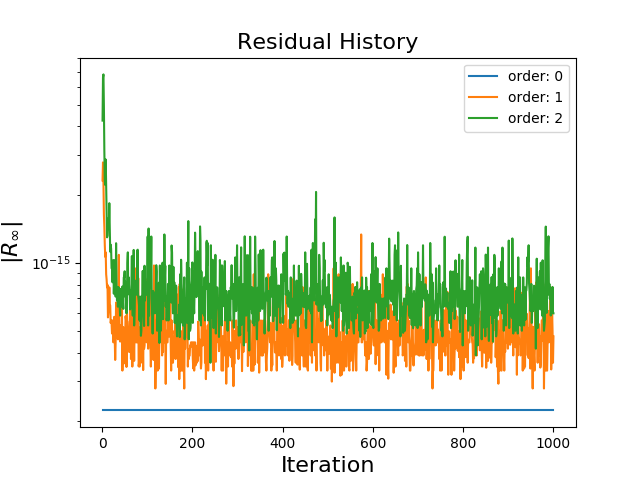
\includegraphics[width=0.60\textwidth,keepaspectratio]{freestream.png}
	\caption{Residual history for the free-stream preservation test}
	\label{fig:free_stream}
\end{figure}


Furthermore we can see when we apply these time marching methods to actual problems that the residual is driven to zero as shown in Figure \ref{fig:res_history}
\begin{figure}[H]
	\centering
	\includegraphics[width=0.60\textwidth,keepaspectratio]{res_history.png}
	\caption{Residual history for \texttt{bump0.gri}}
	\label{fig:res_history}
\end{figure}



\section{Key outputs}

\subsection{Rates of Convergence}

The coefficient of lift ($C_l$), coefficient of drag $(C_d$), and integrated entropy error of the domain (Es) where calculated for each of the five meshes and the convergence of these values can be seen in Figures \ref{fig:conv_cl}, \ref{fig:conv_cd}, and \ref{fig:conv_Es} respectively.
I have included the rate of convergence in each figure for convenience.
In general, the second order method converged toward the exactly value faster than the first order method, but was not also more accurate for each mesh size (error in cl was initially worse).

\begin{figure}[H]
	\centering
	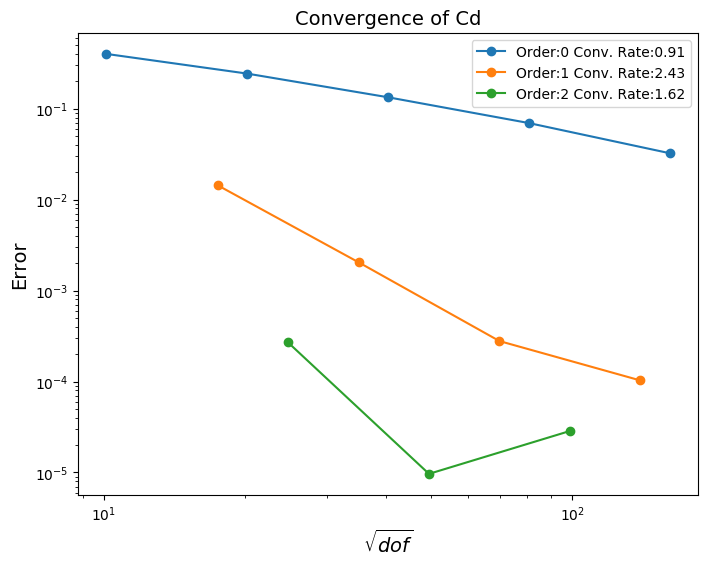
\includegraphics[width=0.60\textwidth,keepaspectratio]{conv_cd.png}
	\caption{The difference between the exact and calculated coefficient of drag decreases with an increasing number elements}
	\label{fig:conv_cl}
\end{figure}
\begin{figure}[H]
	\centering
	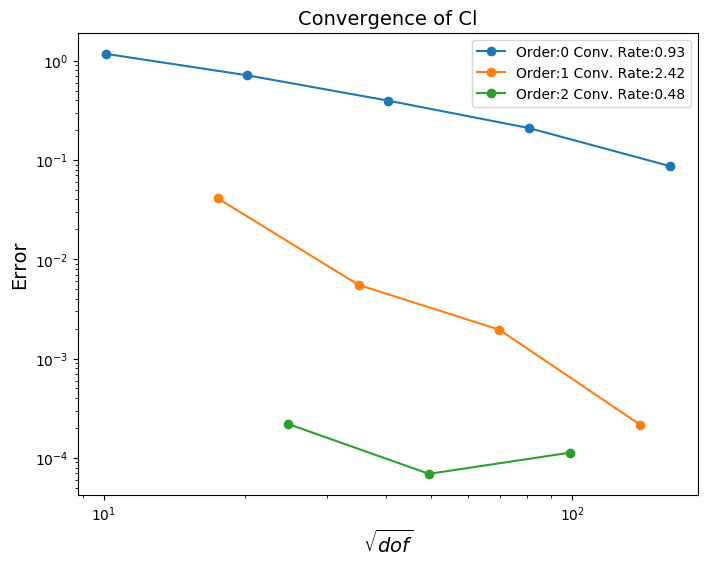
\includegraphics[width=0.60\textwidth,keepaspectratio]{conv_cl.png}
	\caption{The difference between the exact and calculated coefficient of lift decreases with an increasing number elements}
	\label{fig:conv_cd}
\end{figure}
\begin{figure}[H]
	\centering
	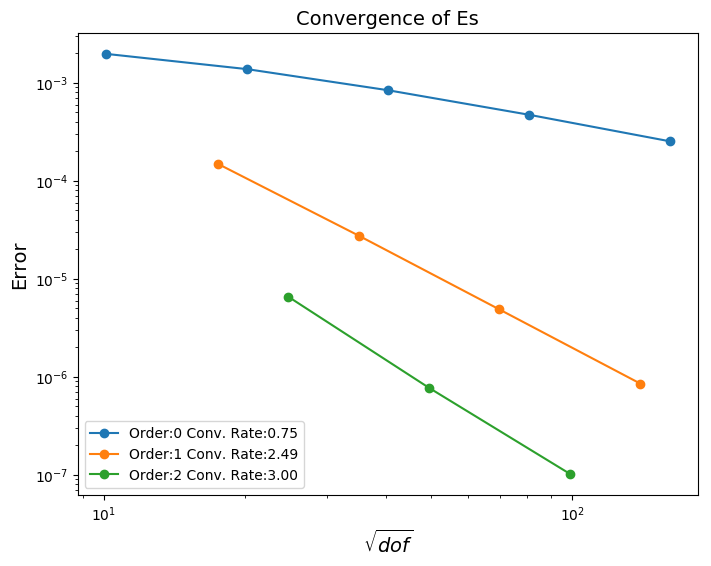
\includegraphics[width=0.60\textwidth,keepaspectratio]{conv_Es.png}
	\caption{The total entropy goes to zero with an increasing number elements}
	\label{fig:conv_Es}
\end{figure}



\subsection{Impact of Reconstruction on Convergence}
During the course of this assignment if was found that for the second-order method reconstructing the state when computing the boundary condition fluxes and when computing the pressure on the wall had a large impact on the overall convergence path for each of the key quantities.
Figure \ref{fig:conv_cl_ex}, \ref{fig:conv_cd_ex}, and \ref{fig:conv_Es_ex} show how  ($C_l$), $(C_d$), and Es converge for each combination of reconstruction.
I elected to reconstruct the states based on $\frac{d\mathbf{u}}{d\mathbf{x}}$ for both the boundary fluxes and when recomputing the pressure along the wall to determine the aerodynamic coefficients (this felt like like the most rigorous thing to do).
Although it should be noted that this choice to use reconstruction for both did not lead to the smoothest convergence plots for my second-order method.


\begin{figure}[H]
	\centering
	\includegraphics[width=0.60\textwidth,keepaspectratio]{conv_cd_ex.png}
	\caption{The convergence of $C_d$ is smoothest without reconstructing the state at the edge in boundary flux Calculations}
	\label{fig:conv_cl_ex}
\end{figure}
\begin{figure}[H]
	\centering
	\includegraphics[width=0.60\textwidth,keepaspectratio]{conv_cl_ex.png}
	\caption{For each of the methods, the convergence of $C_l$ is somewhat jagged}
	\label{fig:conv_cd_ex}
\end{figure}
\begin{figure}[H]
	\centering
	\includegraphics[width=0.60\textwidth,keepaspectratio]{conv_Es_ex.png}
	\caption{The geometry for which the meshes were generated}
	\label{fig:conv_Es_ex}
\end{figure}


\subsection{Pressure Coefficient}
Figure \ref{fig:cp} shows the coefficient of pressure along the lower wall for the \texttt{bump2.gri} mesh.
The second-order method produces a pressure field that is more symmetric on either side of the bump, which we would expect as the exact answer is symmetric.
\begin{figure}[H]
	\centering
	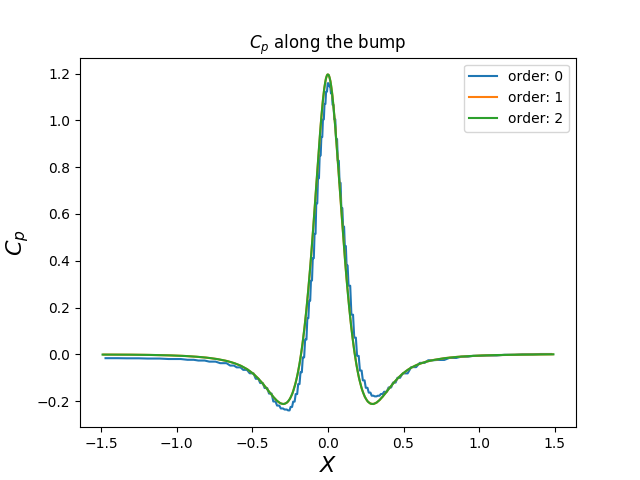
\includegraphics[width=0.60\textwidth,keepaspectratio]{cp.png}
	\caption{The total entropy converges smoothly for all the methods}
	\label{fig:cp}
\end{figure}
\subsection{Mach Contours}
Table \ref{tab:mach} compares the mach field of \texttt{bump2.gri} of the first and second-order methods.
As shown, the second-order method does a better job of preserving the symmetry that you would expect to see in this flow.
This showcases qualitatively how much more accurate the second-order solver is than the first-order solver.
\begin{table}[ht]
	\begin{center}
	\begin{tabular}{ c@{}c@{} }


		\hline
		\multicolumn{2}{@{}c@{}}{First-Order}\\


		\hline
		\multicolumn{2}{@{}c@{}}{\includegraphics[width=0.75\textwidth,keepaspectratio]{machCons_1.png}}\\

		\hline
		\multicolumn{2}{@{}c@{}}{Second-Order}\\

		\hline
		\multicolumn{2}{@{}c@{}}{\includegraphics[width=0.75\textwidth,keepaspectratio]{machCons_2.png}}\\
		\vspace{0.25mm}\\
	\end{tabular}
	\caption{\texttt{bump2.gri} mach contours for each method}
	\label{tab:mach}
	\vspace*{-3mm}
	\end{center}
\end{table}


% \bibliography{references}

\end{document}

